\section{Model Description}
It is the intent of this document to provide a level of understanding of each of the process models sufficient to allow users, with some background of Modelica, the ability to integrate, modify top level parameters, and run simulations of Integrated Energy Systems. Advanced users will be able to use the models as they see fit, but the descriptions provided here will not necessarily explain all facets of the models in detail. 

\subsection{Primary Heat System}
In the Hybrid repository there are four potential primary heat sources: The  Four-Loop PWR plant, the Generic Modular PWR, a natural circulation SMR power plant, and the Natural Gas Fired Turbine. Generally, we consider the Natural Gas Fired Turbine as a peaker unit and thus will save its’ discussion and coverage for the secondary power source section of the Model Descriptions.

\subsubsection{Four Loop Pressurized Water Reactor}

The Four loop PWR system, Figure \ref{Top View Westinghouse}, is designed to be consistent with publicly available information for the Westinghouse plant design \cite{Westinghouse}. This is a Pressurized Water reactor with a nominal thermal power of 3400MWt and has control systems designed to output 1100MWe. All system parameters can be found in the SubSystem model under the “data” record. The steam generator is of U-tube design and operates at a nominal pressure 1000psia. Reactivity feedback can be found in the coreSubchannel module alongside an external source of activity that is designed to provide reactivity feedback from the control rods. Reactivity in the core is based on a point kinetics models, that includes feedback from fission products, boron, fuel temperature, and moderator temperature. System decay heat is calculated from the TRANSFORM package via an eleven-group decay heat correlation from the TRACE user manual.

\begin{figure}[hbtp]
\centering
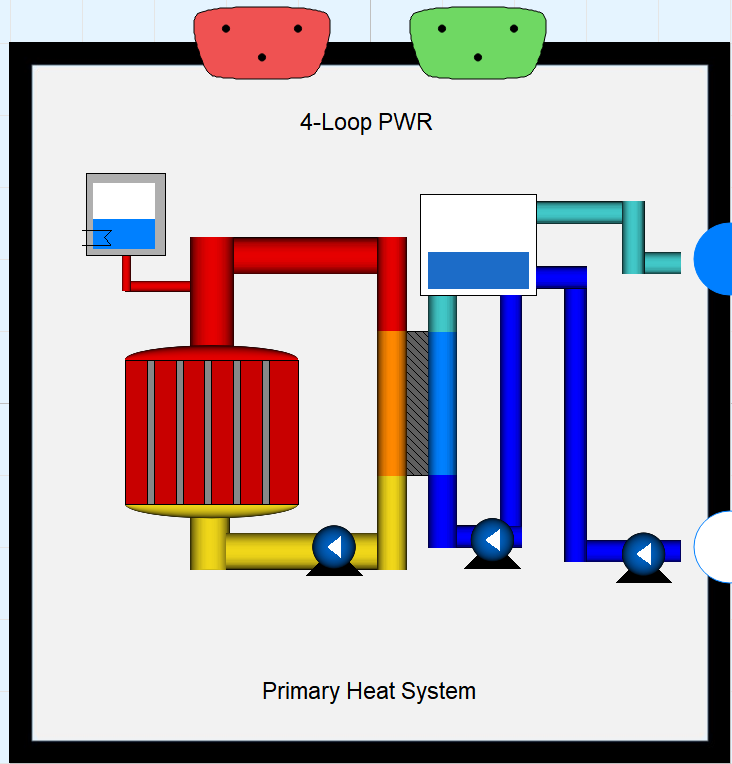
\includegraphics[scale=0.3]{pics/Westinghouse.png}
\caption{Top View of the Four-Loop PWR Plant}
\label{Top View Westinghouse}
\end{figure}


\subsubsection{Generic Modular PWR}
The generic modular PWR unit, Figure \ref{Top View Generic Modular}, is sized to be 160 MWt with 50MWe output as is consistent with the NuScale power module. However, the generic modular PWR does not operate under natural circulation but instead operates under forced flow. Therefore, this unit provides more stability in the code since it does not rely on density differentials to drive flow. This makes the unit less useful than is the NuScale style reactor modeled below, but it does provide the user a power input consistent with NuScale style systems but without the need to tune system geometries, friction factors, etc.. to meet the proper flow dynamics. As with the Westinghouse plant the data file is included in the subsystem  model and has reactivity controls within the core submodule. The Generic Modular PWR relies heavily on the TRANSFORM library for its subcomponents. The steam generator is a once through design with geometrical orientation consistent with a helical coil steam generator. 

\begin{figure}[hbtp]
\centering
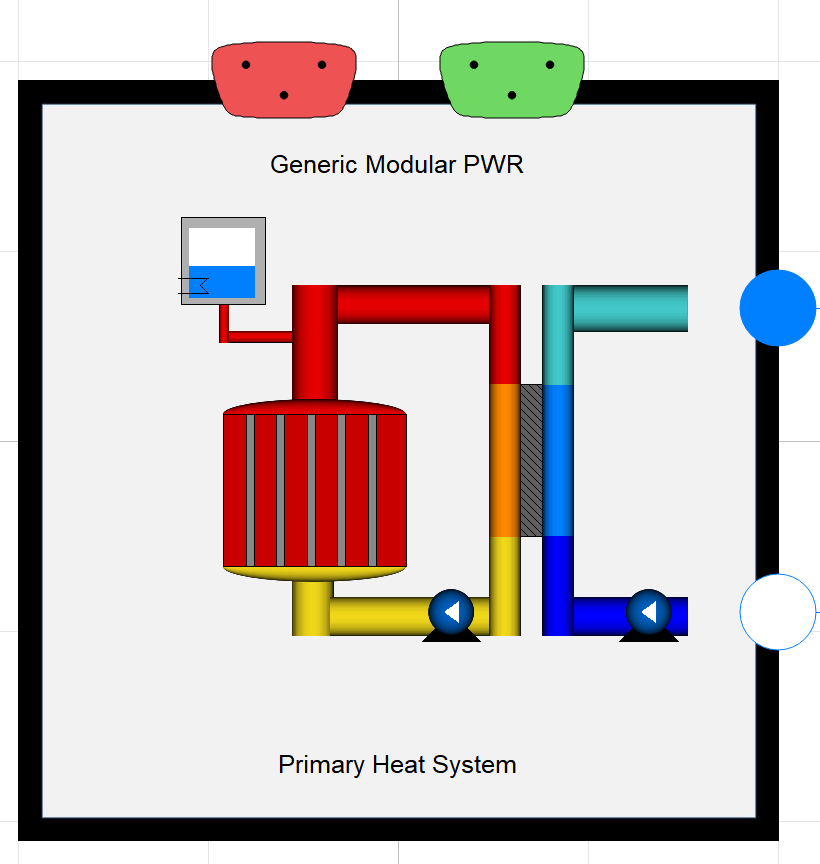
\includegraphics[scale=0.3]{pics/Generic_Modular_PWR.png}
\caption{Top Level Depiction of the Generic Modular PWR in the NHES package.}
\label{Top View Generic Modular}
\end{figure}

% content
\subsubsection{Natural Circulation Small Modular Reactor}
The natural circulation SMR power module,Figure \ref{Top View NuScale Reactor}, is an integral pressurized water reactor (IPWR) that operates with a nominal thermal power of 160 MWt capable of producing 50 MWe to the electric grid. Integral designs are fully self-contained, eliminating the need for large main steam lines that can potentially lead to large break loss of coolant accidents (LOCA). Instead the primary system has only an inlet of feed water into the bottom of the helical coil steam generator and an exit point for steam at the top of the steam generator. All sizes for components is held within the data record in the sub-system. These sizes are consistent with NRC design documentation that can be publicly viewed on the NuScale NRC design certification page. 

The primary system does not include any pumps but instead operates under natural circulation. Natural circulation reactors rely on the height and density differentials between hot and cold water to drive circulation of water through the core. Through elimination of primary coolant pumps an entire class of accident scenarios is eliminated. Modeling efforts in this report focused on three main efforts: matching thermal and electric output, matching system geometry, and matching natural circulation efforts in the system via flow rates and temperature differentials. The primary side of the module has heights and cross-sectional areas in accordance with NRC design certification material. The primary and secondary sides were modeled in their entirety. The helical coil steam generator was modeled as a once through steam generator where the secondary side is on the inside of the tubes and the primary side fluid run along the outside of the tubes.  The full report on this module is available on OSTI \cite{2019NuScaleM4}.


\begin{figure}[hbtp]
\centering
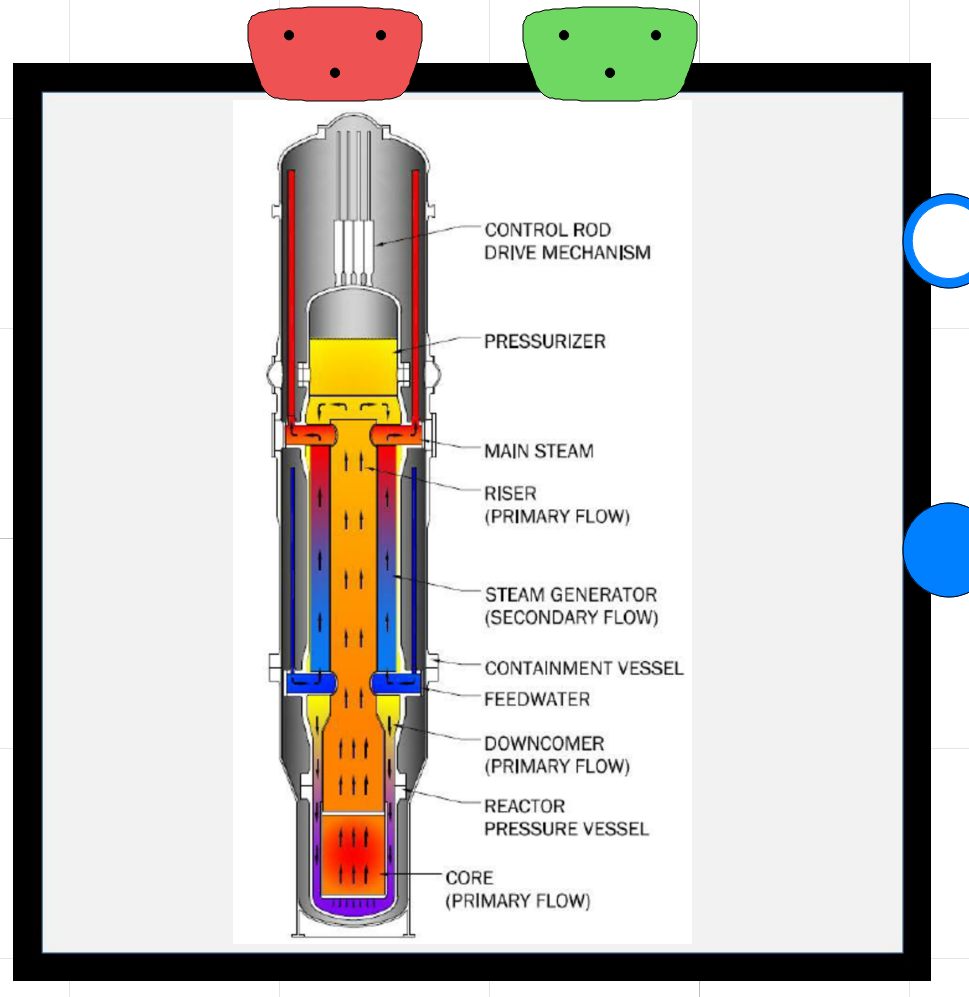
\includegraphics[scale=0.3]{pics/NuScale.png}
\caption{Top Level Depiction of the SMR System in the NHES package.}
\label{Top View NuScale Reactor}
\end{figure}

%\subsection{Cloning the Hybrid Repository}
\label{sec:clone raven}

The first step in installing the package is to clone the HYBRID repository. To do this, use
\begin{lstlisting}[language=bash]
git clone https://github.com/idaholab/HYBRID.git
\end{lstlisting}
This will download the repository into a folder called 'hybrid'. To go inside the folder, use
\begin{lstlisting}[language=bash]
cd hybrid
\end{lstlisting}


\subsubsection{Install RAVEN and its plugins as a sub-module}

The next step is to download and install RAVEN and the submodule (e.g. TEAL, HERON) plugins as a sub-module of the HYBRID repository. 

A submodule allows you to keep another Git repository in a subdirectory of your repository. The other repository has its own history, which does not interfere with the history of the current repository. This can be used to have external dependencies such as third party libraries for example.

In order to get RAVEN do the following in the hybrid folder

\begin{lstlisting}[language=bash]
git checkout devel
\end{lstlisting}

Update the Branch

\begin{lstlisting}[language=bash]
git pull
\end{lstlisting}

to add RAVEN as a submodule
\begin{lstlisting}[language=bash]
git submodule update --init --recursive
\end{lstlisting}

\textbf{Install and Compile RAVEN. }
Once you have downloaded RAVEN as a sub-module, you have to install it. go to the \href{https://github.com/idaholab/raven/wiki/intallationMain}{RAVEN Wiki} for information about how to install it. Run all the tests outlined in the RAVEN wiki. 

\subsubsection{Inform the Framework Paths}

In order to set up the hybrid repository, you must inform the framework about the location of the Dymola python interface. For doing so, navigate to the hybrid directory:

to add RAVEN as a submodule
\begin{lstlisting}[language=bash]
cd <path to your hybrid repository>/hybrid
\end{lstlisting}
Run the following command:
\begin{lstlisting}[language=bash]
./scripts/write_hybridrc.py -p DYMOLA_PATH
\end{lstlisting}

Where DYMOLAPATH is the path to the python interface egg folder in the DYMOLA installation locally. For example:
 
\begin{lstlisting}[language=bash]
./scripts/write_hybridrc.py -p 
	"/c/Program\ Files/Dymola\ 2020x/Modelica/Library/
	python_interface/dymola.egg"
\end{lstlisting}

